%----------------------------------------------------------------------------------------
%	PACKAGES AND OTHER DOCUMENT CONFIGURATIONS
%----------------------------------------------------------------------------------------

\documentclass{article}
\usepackage{xeCJK} %调用 xeCJK 宏包
\setCJKmainfont{STSong} %设置 CJK 主字体为 SimSun (宋体)
%\setCJKmainfont[BoldFont=STZhongsong]{STSong}
\setCJKsansfont[BoldFont=STHeiti]{STXihei}
\setCJKmonofont{STFangsong}
\usepackage{fancyhdr} % Required for custom headers
\usepackage{lastpage} % Required to determine the last page for the footer
\usepackage{extramarks} % Required for headers and footers
\usepackage[usenames,dvipsnames]{color} % Required for custom colors
\usepackage{graphicx} % Required to insert images
\usepackage{listings} % Required for insertion of code
\usepackage{courier} % Required for the courier font
\usepackage{lipsum} % Used for inserting dummy 'Lorem ipsum' text into the template
\usepackage{booktabs}
\usepackage{multirow}

% Margins
\topmargin=-0.45in
\evensidemargin=0in
\oddsidemargin=0in
\textwidth=6.5in
\textheight=9.0in
\headsep=0.25in

\linespread{1.3} % Line spacing

% Set up the header and footer
\pagestyle{fancy}
\lhead{\hmwkAuthorName\ \hmwkAuthorNumber} % Top left header
\chead{\hmwkClass\ : \hmwkTitle} % Top center head
\rhead{\firstxmark} % Top right header
\lfoot{\lastxmark} % Bottom left footer
\cfoot{} % Bottom center footer
\rfoot{Page\ \thepage\ of\ \protect\pageref{LastPage}} % Bottom right footer
\renewcommand\headrulewidth{0.4pt} % Size of the header rule
\renewcommand\footrulewidth{0.4pt} % Size of the footer rule

\setlength\parindent{0pt} % Removes all indentation from paragraphs

%----------------------------------------------------------------------------------------
%	CODE INCLUSION CONFIGURATION
%----------------------------------------------------------------------------------------

\definecolor{MyDarkGreen}{rgb}{0.0,0.4,0.0} % This is the color used for comments
\lstloadlanguages{Python} % Load Perl syntax for listings, for a list of other languages supported see: ftp://ftp.tex.ac.uk/tex-archive/macros/latex/contrib/listings/listings.pdf
\lstset{language=Python, % Use Python in this example
        frame=single, % Single frame around code
        basicstyle=\small\ttfamily, % Use small true type font
        keywordstyle=[1]\color{Blue}\bf, % Perl functions bold and blue
        keywordstyle=[2]\color{Purple}, % Perl function arguments purple
        keywordstyle=[3]\color{Blue}\underbar, % Custom functions underlined and blue
        identifierstyle=, % Nothing special about identifiers                                         
        commentstyle=\usefont{T1}{pcr}{m}{sl}\color{MyDarkGreen}\small, % Comments small dark green courier font
        stringstyle=\color{Purple}, % Strings are purple
        showstringspaces=false, % Don't put marks in string spaces
        tabsize=5, % 5 spaces per tab
        %
        % Put standard Perl functions not included in the default language here
        morekeywords={rand},
        %
        % Put Perl function parameters here
        morekeywords=[2]{on, off, interp},
        %
        % Put user defined functions here
        morekeywords=[3]{test},
       	%
        morecomment=[l][\color{Blue}]{...}, % Line continuation (...) like blue comment
        numbers=left, % Line numbers on left
        firstnumber=1, % Line numbers start with line 1
        numberstyle=\tiny\color{Blue}, % Line numbers are blue and small
        stepnumber=5 % Line numbers go in steps of 5
}

\newcommand{\pythonscript}[2]{
\begin{itemize}
\item[]\lstinputlisting[caption=#2,label=#1]{#1.py}
\end{itemize}
}

%----------------------------------------------------------------------------------------
%	DOCUMENT STRUCTURE COMMANDS
%	Skip this unless you know what you're doing
%----------------------------------------------------------------------------------------

% Header and footer for when a page split occurs within a problem environment
\newcommand{\enterProblemHeader}[1]{
\nobreak\extramarks{#1}{#1 continued on next page\ldots}\nobreak
\nobreak\extramarks{#1 (continued)}{#1 continued on next page\ldots}\nobreak
}

% Header and footer for when a page split occurs between problem environments
\newcommand{\exitProblemHeader}[1]{
\nobreak\extramarks{#1 (continued)}{#1 continued on next page\ldots}\nobreak
\nobreak\extramarks{#1}{}\nobreak
}

\setcounter{secnumdepth}{0} % Removes default section numbers
\newcounter{homeworkProblemCounter} % Creates a counter to keep track of the number of problems

\newcommand{\homeworkProblemName}{}
\newenvironment{homeworkProblem}[1][Problem \arabic{homeworkProblemCounter}]{ % Makes a new environment called homeworkProblem which takes 1 argument (custom name) but the default is "Problem #"
\stepcounter{homeworkProblemCounter} % Increase counter for number of problems
\renewcommand{\homeworkProblemName}{#1} % Assign \homeworkProblemName the name of the problem
\section{\homeworkProblemName} % Make a section in the document with the custom problem count
\enterProblemHeader{\homeworkProblemName} % Header and footer within the environment
}{
\exitProblemHeader{\homeworkProblemName} % Header and footer after the environment
}

\newcommand{\problemAnswer}[1]{ % Defines the problem answer command with the content as the only argument
\noindent\framebox[\columnwidth][c]{\begin{minipage}{0.98\columnwidth}#1\end{minipage}} % Makes the box around the problem answer and puts the content inside
}

\newcommand{\homeworkSectionName}{}
\newenvironment{homeworkSection}[1]{ % New environment for sections within homework problems, takes 1 argument - the name of the section
\renewcommand{\homeworkSectionName}{#1} % Assign \homeworkSectionName to the name of the section from the environment argument
\subsection{\homeworkSectionName} % Make a subsection with the custom name of the subsection
\enterProblemHeader{\homeworkProblemName\ [\homeworkSectionName]} % Header and footer within the environment
}{
\enterProblemHeader{\homeworkProblemName} % Header and footer after the environment
}

%----------------------------------------------------------------------------------------
%	NAME AND CLASS SECTION
%----------------------------------------------------------------------------------------

\newcommand{\hmwkTitle}{Assignment\ \#4} % Assignment title
\newcommand{\hmwkClass}{人工智能导论} % Course/class
\newcommand{\hmwkAuthorName}{张知行} % Your name
\newcommand{\hmwkAuthorNumber}{2015012018}

%----------------------------------------------------------------------------------------
%	TITLE PAGE
%----------------------------------------------------------------------------------------

\title{
\vspace{2in}
\textmd{\textbf{\hmwkClass:\ \hmwkTitle}}\\
\vspace{3in}
}

\author{\textbf{\hmwkAuthorName\ \hmwkAuthorNumber}}
%\textit{\hmwkAuthorNumber}
\date{\today} % Insert date here if you want it to appear below your name

%----------------------------------------------------------------------------------------

\begin{document}

\maketitle

%----------------------------------------------------------------------------------------
%	TABLE OF CONTENTS
%----------------------------------------------------------------------------------------

%\setcounter{tocdepth}{1} % Uncomment this line if you don't want subsections listed in the ToC

\newpage
%\tableofcontents
%\newpage

\begin{homeworkProblem}[Value Iteration]
	\paragraph{}
	Description: Write a value iteration agent in ValueIterationAgent, which has been partially specified in valueIterationAgents.py. ValueIterationAgent agent is an offline planner, not a reinforcement learning agent, and so the relevant training option is the number of iterations of value iteration it should run (option -i) in its initial planning phase. 
	\paragraph{}
	由于实现的$ValueIterationAgent$是一个离线的算法,因此需要在初始化的时候对后续所有情况进行计算并进行存储。在每次迭代中,计算所有状态下的$QValue$,使用最后的$QValue$以及记录下的每个状态下最好的操作方式作为最终的结果来对$agent$进行操作。每个格点上的$Value$是在该格点所有可能动作下$QValue$的最大值,同样,在该格点处选择的操作也是$QValue$最大的操作对应的值。使用100次迭代计算得到的结果如Figure\ref{q1value}和Figure\ref{q1QValue}所示。
	\begin{figure}[ht]
		\centering
		\begin{minipage}[t]{0.4\textwidth}
		\centering
		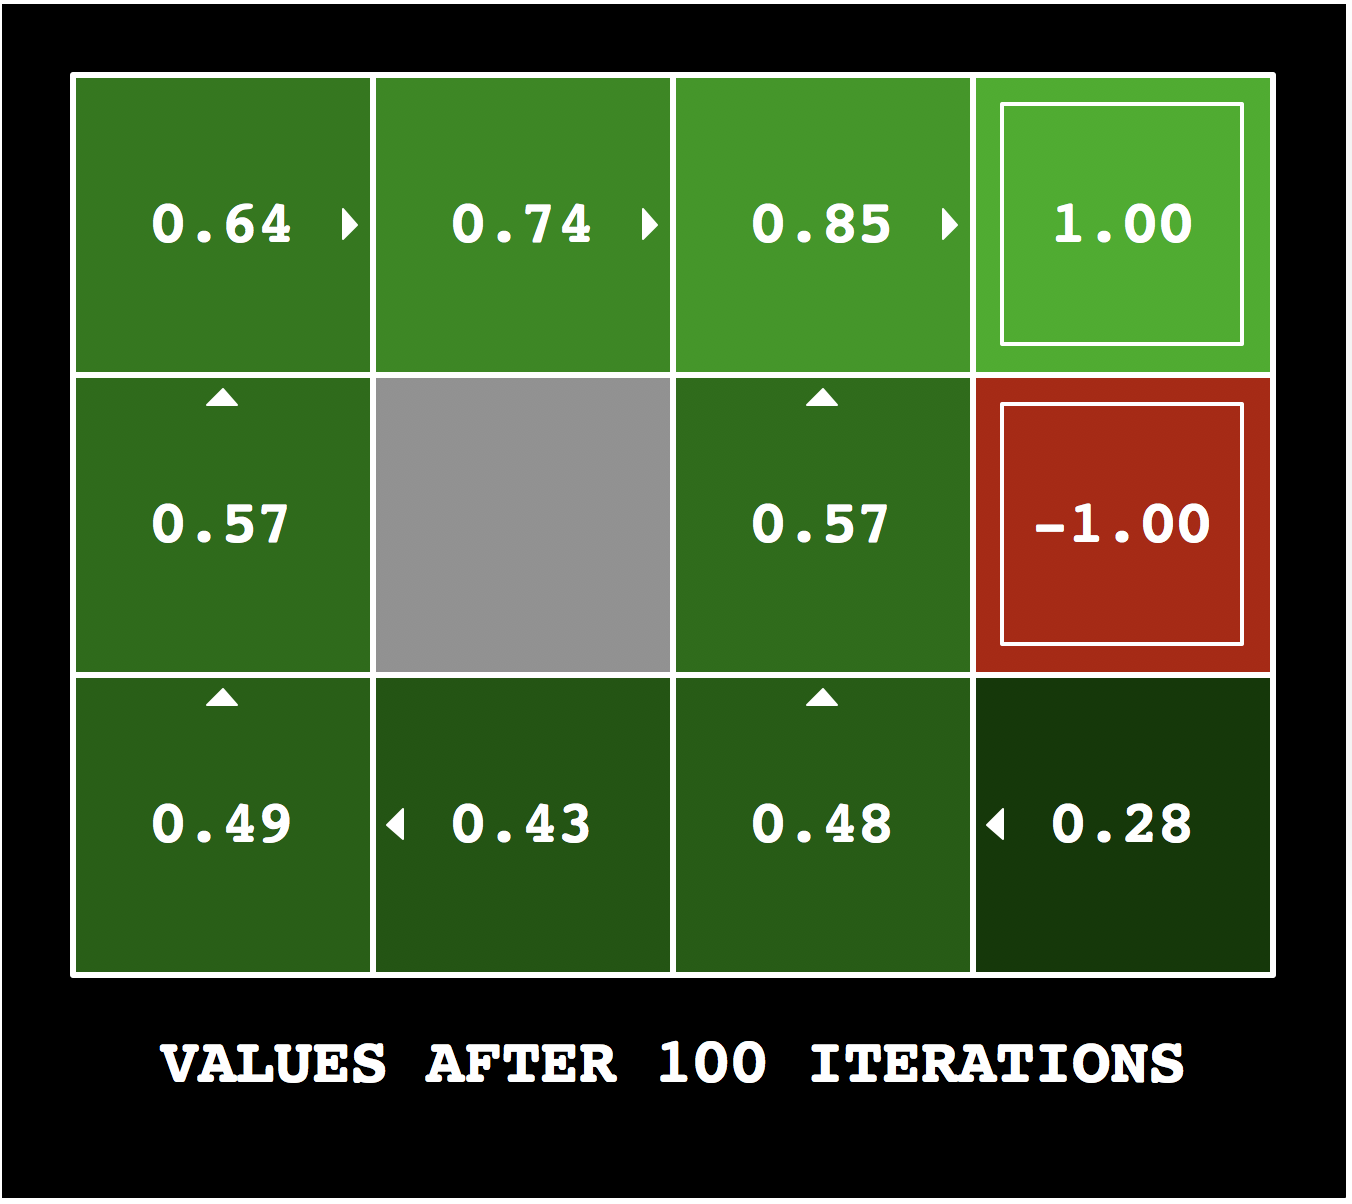
\includegraphics[width=6cm]{q1_100_Value.png}
		\caption{Values after 100 iterations}
		\label{q1value}
		\end{minipage}
		\centering
		\begin{minipage}[t]{0.4\textwidth}
		\centering
		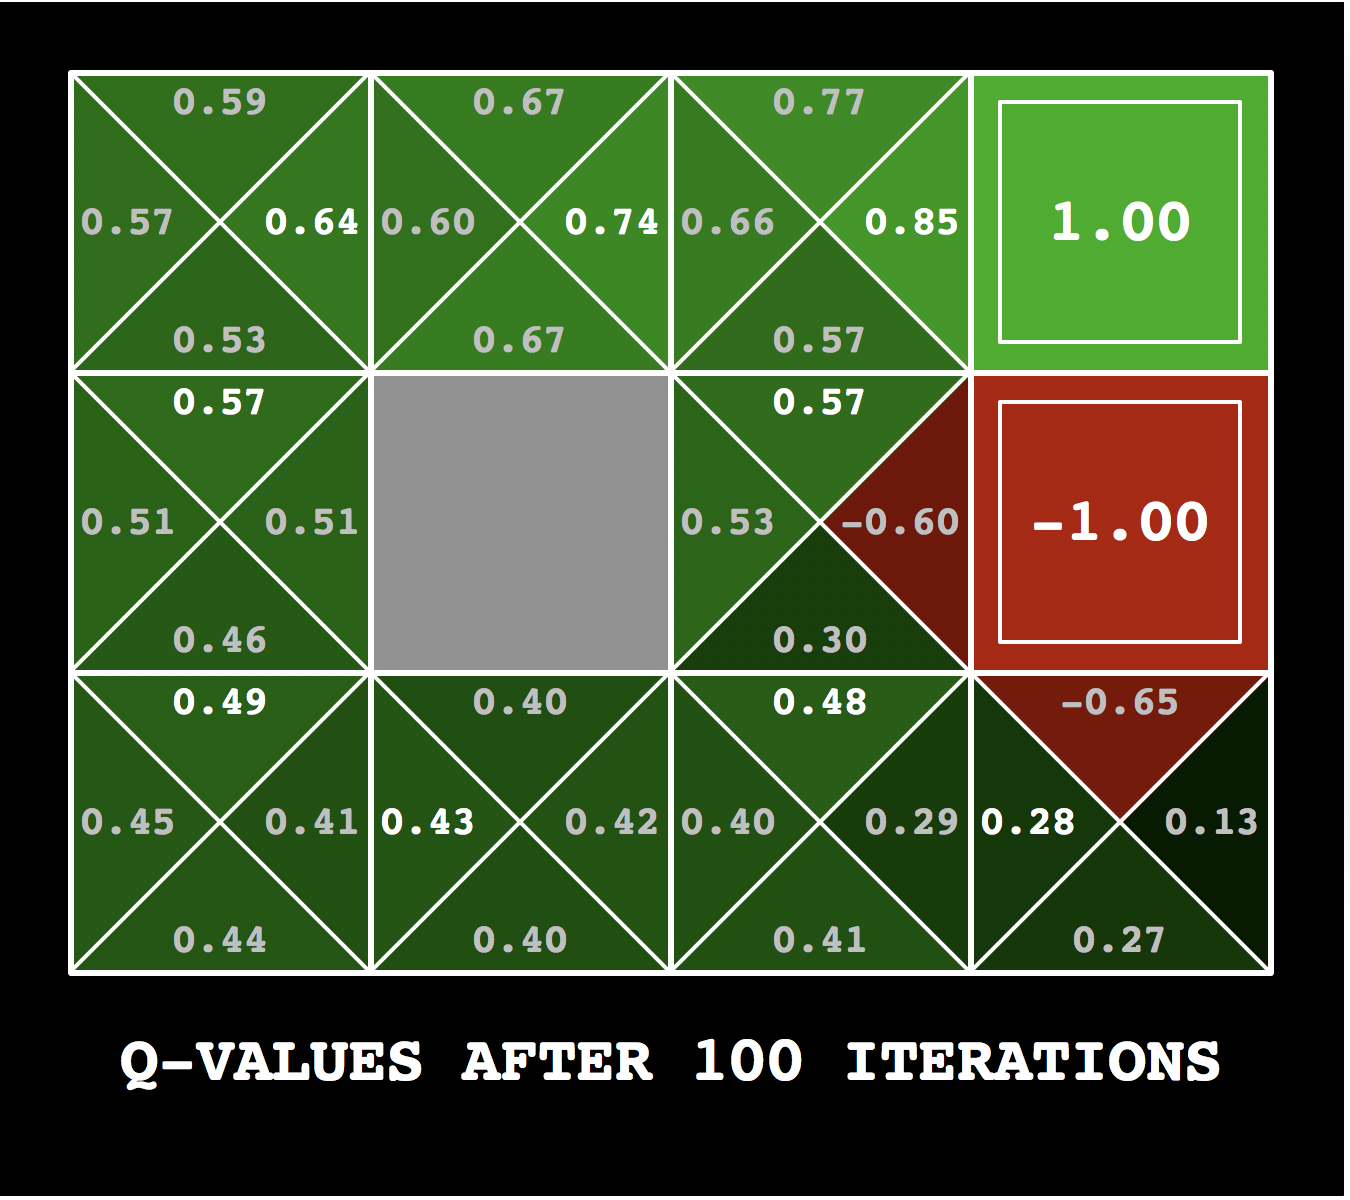
\includegraphics[width=6cm]{q1_100_QValues.png}
		\caption{QValues after 100 iterations}
		\label{q1QValue}
		\end{minipage}
		\centering
	\end{figure}
	\paragraph{}
	其余设定不变,分别进行100次和5次迭代之后进行10次测试得到的结果,如Figure\ref{q1100}和Figure\ref{q15}所示。可以看出增加迭代次数会减少错误率,更好地实现路径规划。
	\begin{figure}[ht]
		\centering
		\begin{minipage}[t]{0.4\textwidth}
		\centering
		
\includegraphics[width=6cm]{q1_100_return.png}
		\caption{Returns after 100 iterations}
		\label{q1100}
		\end{minipage}
		\centering
		\begin{minipage}[t]{0.4\textwidth}
		\centering
		
\includegraphics[width=6cm]{q1_5_return.png}
		\caption{Returns after 5 iterations}
		\label{q15}
		\end{minipage}
		\centering
	\end{figure}
\end{homeworkProblem}

\begin{homeworkProblem}[Parameter Analysis in Value Iteration]
	\paragraph{}
	Description: Change parameters so that the optimal policy causes the agent to attempt to cross the bridge.
	\paragraph{}
	这一问中需要深入理解第一问中实现的$ValueIterationAgent$的具体的参数的功能。在初始的参数设定下,agent会通过局部较好的情况走向分数较小的最终结果,需要改变参数中的$Discount$或者$Noise$的数值来实现Agent更为长远的考虑。从$ValueIterationAgent$中使用的计算$QValue$的公式来看,对于越远的位置,由于discount造成的影响越大,造成下一步中计算得到向该方向前进的可能性越小,但是初始的$discount$的数值为$0.9$可以向上调整的幅度不大,并且经过测试,过大的$discount$会造成选择特别差的路径。因此对$Noise$进行修改。通过修改,发现将$Noise$降低到$0.02$之后会很大程度上降低向左的数值,但是仍然会有走向低分的规划。最终测试结果发现$Noise = 0.001$可以很好地实现要求的结果,最终结果如Figure\ref{q2}。
	\begin{figure}[ht]
		\centering
		\begin{minipage}[t]{0.7\textwidth}
		\centering
		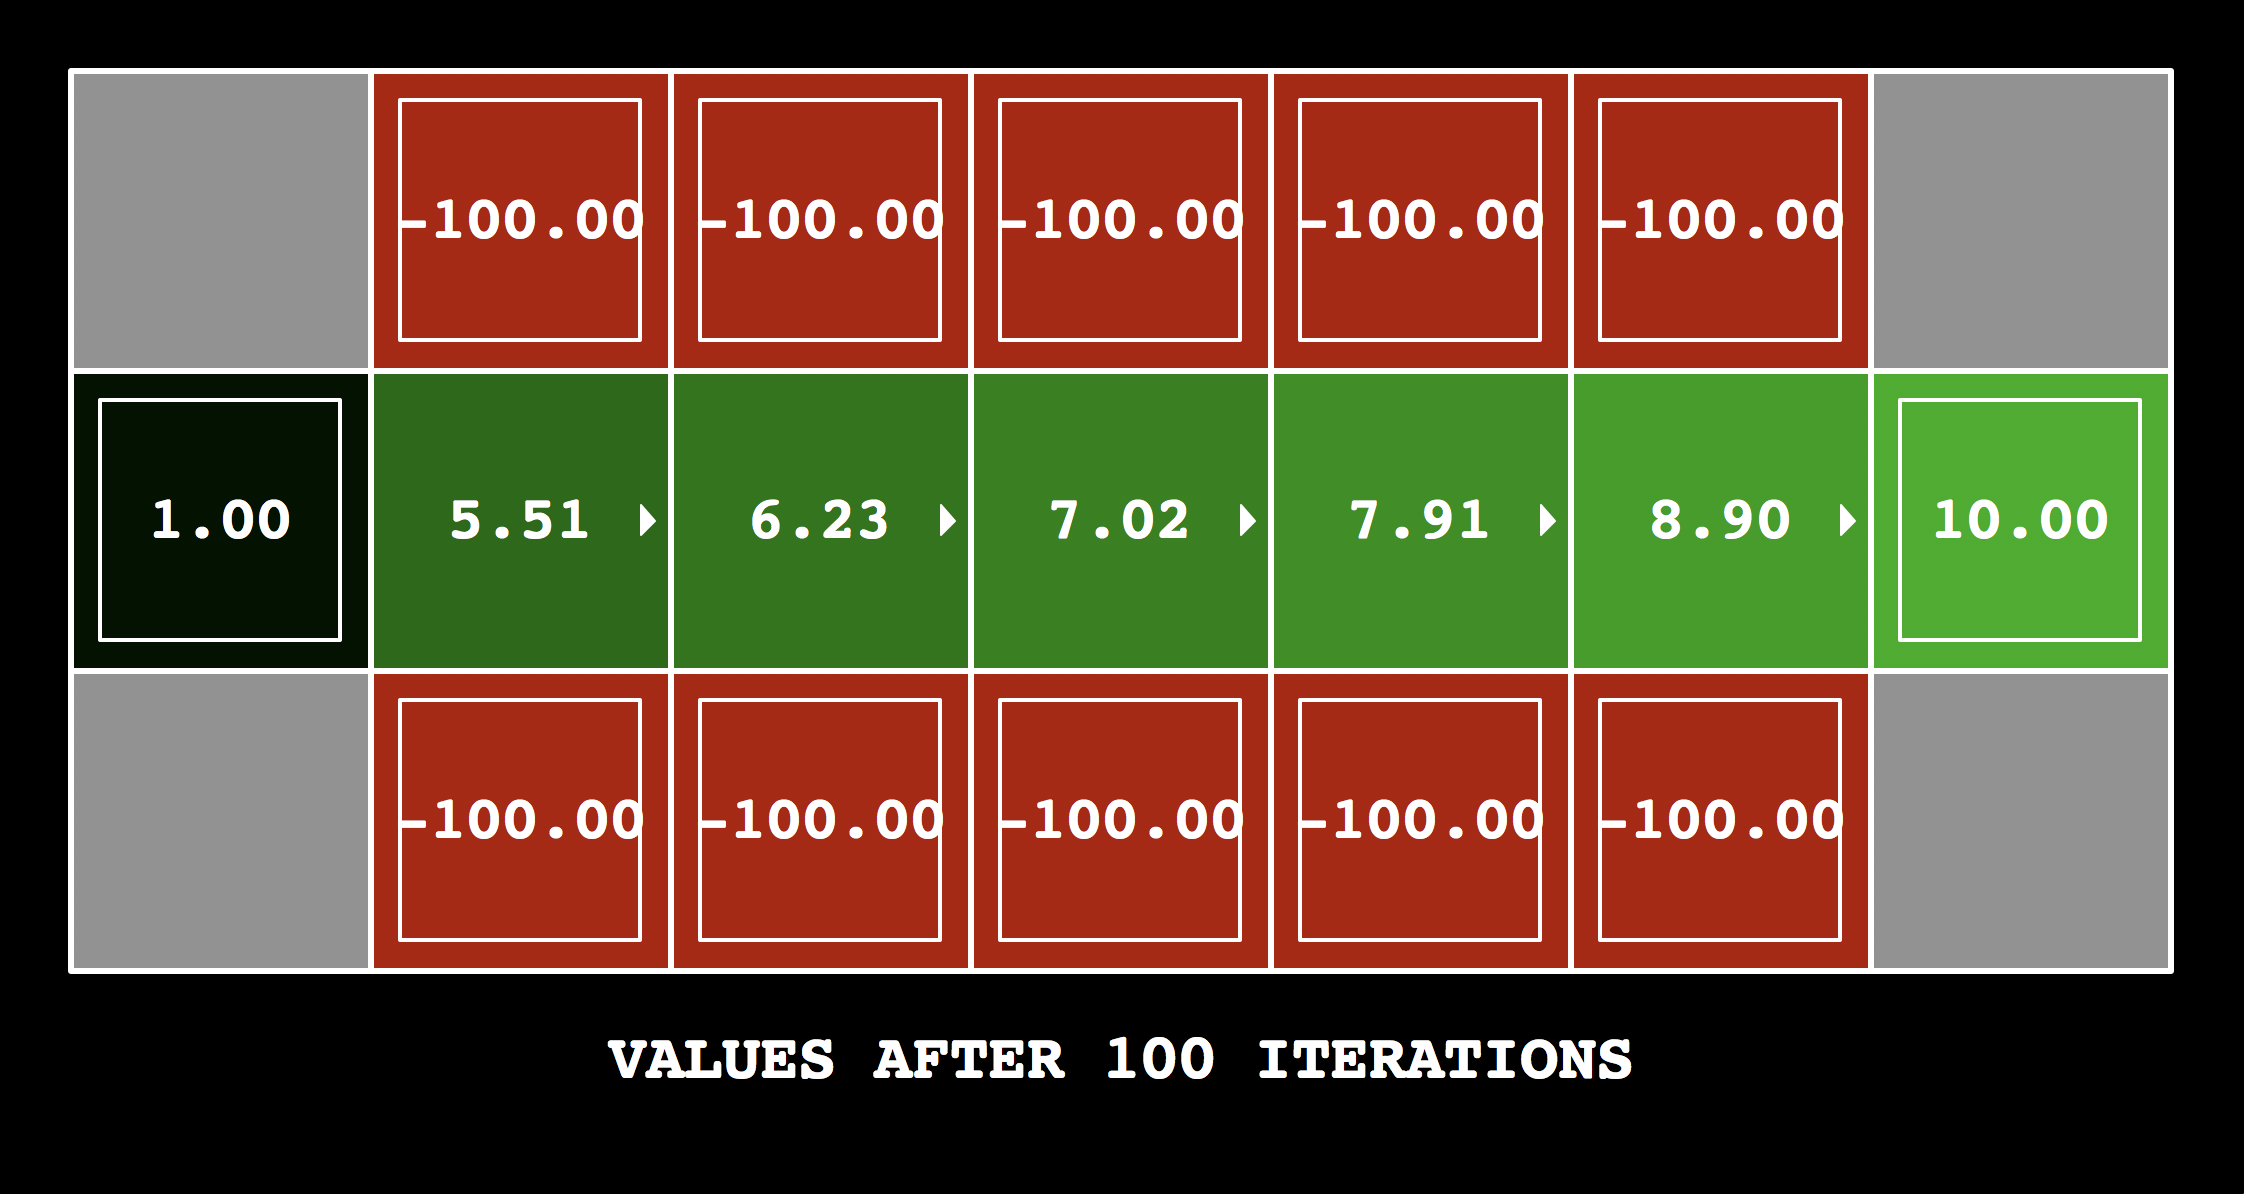
\includegraphics[width=12cm]{q2.png}
		\caption{Values after 100 iterations}
		\label{q2}
		\end{minipage}
		\centering
	\end{figure}
\end{homeworkProblem}

\begin{homeworkProblem}[Q-Learning]
	\begin{figure}[ht]
		\centering
		\begin{minipage}[t]{0.4\textwidth}
		\centering
		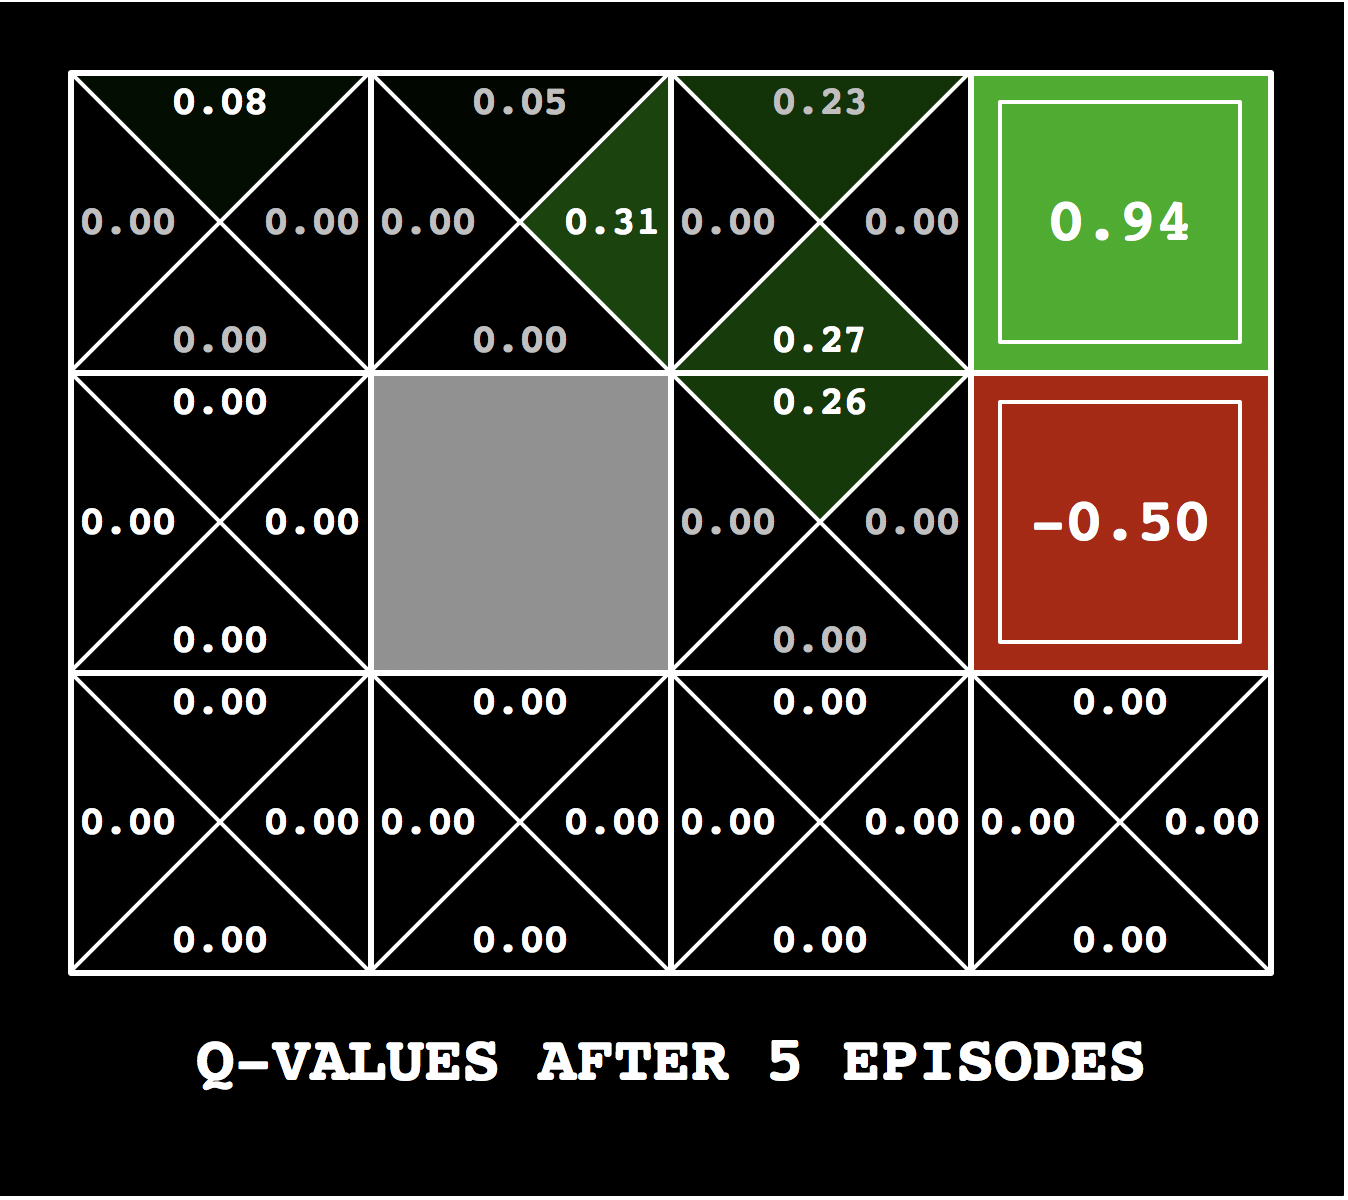
\includegraphics[width=6cm]{q4_5.png}
		\caption{Values after 5 episodes}
		\label{q4_5}
		\end{minipage}
		\centering
		\begin{minipage}[t]{0.4\textwidth}
		\centering
		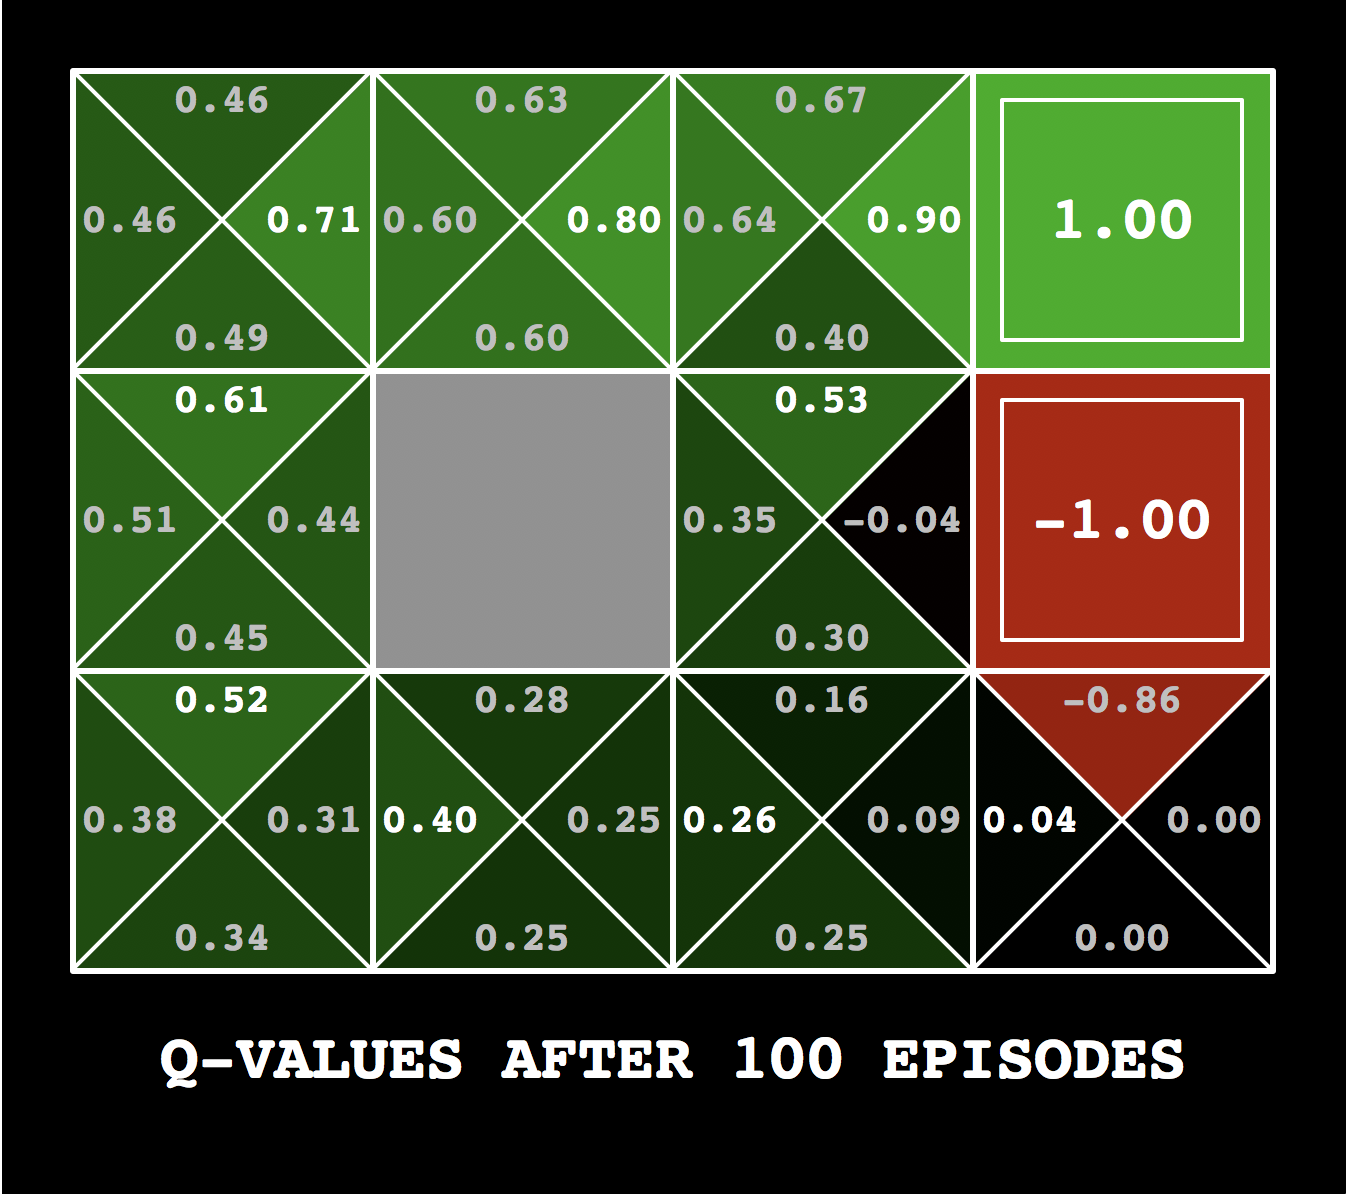
\includegraphics[width=6cm]{q4_100.png}
		\caption{Values after 100 episodes}
		\label{q4_100}
		\end{minipage}
		\centering
		\begin{minipage}[t]{0.4\textwidth}
		\centering
		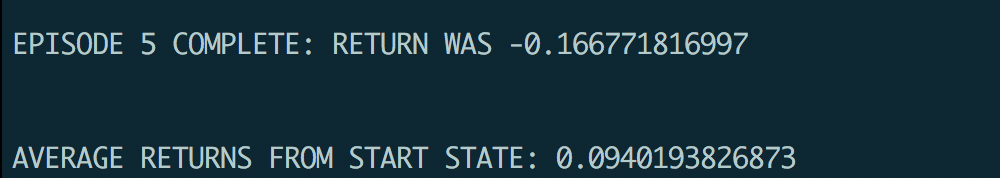
\includegraphics[width=6cm]{q4_5_r.png}
		\caption{Results after 5 episodes}
		\label{q4_5_r}
		\end{minipage}
		\centering
		\begin{minipage}[t]{0.4\textwidth}
		\centering
		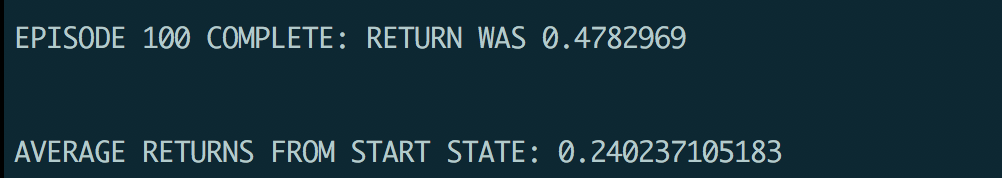
\includegraphics[width=6cm]{q4_100_r.png}
		\caption{Results after 5 episodes}
		\label{q4_100_r}
		\end{minipage}
		\centering
	\end{figure}

	\paragraph{}
	Description: Implement the update, computeValueFromQValues, getQValue, computeActionFromQValues methods in QLearningAgent in qlearningAgents.py.
	\paragraph{}
	这一问中需要对$QLearning$进行实现,是一个通过不断的实践进行学习的算法,核心主要在$update$过程中,当前状态进行一个动作对应的$QValue$是之前同样情况下进行相同操作的$QValue$的数值和下一个状态下之前经验的一个组合。分别使用5次训练和100次训练查看结果如Figure\ref{q4_5},\ref{q4_100},\ref{q4_5_r},\ref{q4_100_r}。可以看出通过大量的训练测试结果有了很好地提升。
	\end{homeworkProblem}

\begin{homeworkProblem}[Q-Learning and Pacman]
	\paragraph{}
	这一问中要求修改$QLearningAgent$使其可以适配于PacMan的操作,通过测试,发现上一问中实现的代码可以很好地适用于这一问中的测试中,$autograder$测试结果如Figure \ref{q5}。同时,通过测试可以发现,在较小的Grid下PacMan可以有很好地表现。但是,如果使用较大的Grid,PacMan则会出现静止不动的现象,最终会造成失败,主要原因可能是状态过多,学习效果较差,PacMan无法分辨Ghost的危险。因此这种算法并不具有大规模下使用的能力。
	\begin{figure}[ht]
		\centering
		\begin{minipage}[t]{0.4\textwidth}
		\centering
		
\includegraphics[width=6cm]{q5.png}
		\caption{Autograder result}
		\label{q5}
		\end{minipage}
		\centering
	\end{figure}
\end{homeworkProblem}

\begin{homeworkProblem}[Approximate Q-Learning]
	\paragraph{}
	Description: Implement an approximate Q-learning agent that learns weights for features of states.
	\paragraph{}
	这一问需要使用特征提取函数进行学习,从而可以实现更好的学习效果,和上一问中最大的区别是使用提取出来的特征作为字典的key值而不是(state, action)的二元组。使用这种学习方法可以看出有着较好的学习效果,很好地解决了上一问中PacMan在较大的地图下无法进行判断的问题。最终结果使用各种地图进行测试几乎都会得到胜利的结果,$autograder$测试结果如Figure \ref{q6}。
	\begin{figure}[ht]
		\centering
		\begin{minipage}[t]{0.4\textwidth}
		\centering
		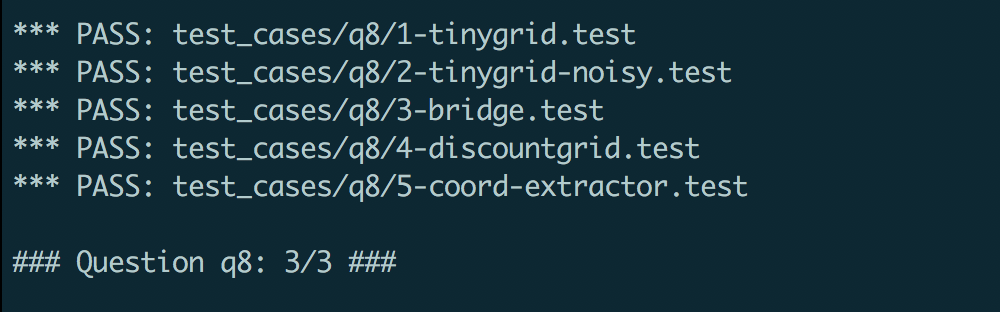
\includegraphics[width=6cm]{q6.png}
		\caption{Autograder result}
		\label{q6}
		\end{minipage}
		\centering
	\end{figure}
\end{homeworkProblem}
\end{document}